\RequirePackage[hyphens]{url}

\documentclass[sigconf]{acmart}

\usepackage{graphicx}
\usepackage{hyperref}
\usepackage{todonotes}

\usepackage{endfloat}
\renewcommand{\efloatseparator}{\mbox{}} % no new page between figures

\usepackage{booktabs} % For formal tables

\settopmatter{printacmref=false} % Removes citation information below abstract
\renewcommand\footnotetextcopyrightpermission[1]{} % removes footnote with conference information in first column
\pagestyle{plain} % removes running headers

\newcommand{\TODO}[1]{\todo[inline]{#1}}

\begin{document}

\title{Income Prediction based on Machine Learning Techniques}

\author{Borga Edionse Usifo}
\affiliation{%
\institution{Indiana University}
\city{Bloomington} 
\state{Indiana} 
\postcode{47408}
}
\email{busifo@iu.edu}

\renewcommand{\shortauthors}{B. Usifo et al.}

\begin{abstract}
This project takes a closer look to some of the most used supervised learning algorithms in machine learning. We start with the description of the each of the algorithms then we move it to analytics and findings by using that particular algorithm in our data-set. We also provide advantages and disadvantages of each supervised machine learning algorithm for future reference. We mainly focus on our prediction of the income level of individuals by looking at their age, gender, education, location, and other features given by our data-set. We will try each algorithm and try to pick the best features from our data-set to have an optimal prediction.
\end{abstract}

\keywords{i523, HID343, Machine Learning, Income Prediction, Logistic Regression, Ensemble methods}

\maketitle
%%%%%%%%%%%%%%%%%%%%%%%%%%%%%%%%%%%%%%%%%%%%%%%%%%%%%%%%%%%%%%%%%%%%%%%%%%%%%%%%%%%%%%%%%%%%%%%%%%%%%%%%%%%%%%%%%%%%%%%%%%%%%%%%%%%%%%%%%%%%%%%%%%%%%%%%%

\section{Introduction}

In this project, we try to showcase the performance of the machine learning algorithms on data which we gather from UCI machine learning repository \cite{www-uci}. This data used by Kohavi R. and Becker B. for their research in improving the in Naive Bayes Classifier's accuracy \cite{Kohavi:1996:SUA:3001460.3001502}. 
\par Data consists of 15 variables, and we try to predict the income of the individuals. To do this prediction task, we first started with data preparation because the data we receive from UCI machine learning repository \cite{www-uci} not fully prepared for any machine learning algorithm. Our first task was the clean the data while applying some statistical techniques to get insights from the dataset. We also used data transformation methods like One-Hot-Encoding\cite{www-hackernoon} to apply logarithmic functions for improving the machine learning algorithms performance before training the data. 
\par Machine Learning algorithms that we discuss in this paper are Gaussian Naive Bayes \cite{www-wikipedia-naivebayes}, K Nearest Neighbors \cite{Lee2017-knn}, Ensemble Methods (Boosting) \cite{dietterich-ensemble}, Support Vector Machines \cite{www-simafore-svm}, Logistic Regression \cite{adarsh}, and Decision Trees \cite{www-wikipedia.decision}. We try to show their weakness, advantages, and their time consumption while training each of them in machine learning algorithms section. 
\par After providing a brief introduction of each of the supervised machine learning algorithms, we will discuss our findings for of each of the algorithms by comparing their accuracy score, F-1 score, recall, and lastly time comparison. 

%%%%%%%%%%%%%%%%%%%%%%%%%%%%%%%%%%%%%%%%%%%%%%%%%%%%%%%%%%%%%%%%%%%%%%%%%%%%%%%%%%%%%%%%%%%%%%%%%%%%%%%%%%%%%%%%%%%%%%%%%%%%%%%%%%%%%%%%%%%%%%%%%%%%%%%%%

\section{Importance of Big Data Analytics for Predictive CLassification}

Importance of big data analytics is getting higher every day since the algorithms become more powerful to predict, classify and cluster any given data set. Importance of our case is any company can be used to predict individuals income to refer them goods in their income range or governments can provide additional support for the areas that have lower income range. There can be many possible things that can do with this kind of classification predictions. 

%%%%%%%%%%%%%%%%%%%%%%%%%%%%%%%%%%%%%%%%%%%%%%%%%%%%%%%%%%%%%%%%%%%%%%%%%%%%%%%%%%%%%%%%%%%%%%%%%%%%%%%%%%%%%%%%%%%%%%%%%%%%%%%%%%%%%%%%%%%%%%%%%%%%%%%%%

\section{Data Preparation}

We first used the pandas \cite{www-pandas} to help to load the data in data frame format. This gave us a unique advantage, and faster processing of comma separated values for putting into data frame \cite{www-commasep}.  Our data consist of 15 variables. Some of these variables are continuous, and some of them are categorical variables, and our target variable was ``income`` attribute. After putting the data into data frames, we first got a statistical snapshot of continuous variables ( age, education, capital gain, capital loss, hours worked) by using the pandas \cite{www-pandas.describe} functions as shown in Table \ref{stats-table}. 

\begin{table}[!ht]
\centering
\begin{tabular}{|l|l|l|l|l|l|}
\hline
               & \textbf{age} & \textbf{education} & \textbf{cap gain} & \textbf{cap loss} & \textbf{hours} \\ \hline
\textbf{count} & 32561        & 32561              & 32561             & 32561             & 32561          \\ \hline
\textbf{mean}  & 38.581       & 10.08              & 1077.64           & 87.303            & 40.437         \\ \hline
\textbf{std.}  & 13.640       & 2.572              & 7385.292          & 402.960           & 12.347         \\ \hline
\textbf{min.}  & 17.0         & 1.0                & 0                 & 0                 & 1.0            \\ \hline
\textbf{25\%}  & 28.0         & 9.0                & 0                 & 0                 & 40.0           \\ \hline
\textbf{50\%}  & 37.0         & 10.0               & 0                 & 0                 & 40.0           \\ \hline
\textbf{75\%}  & 48.0         & 12.0               & 0                 & 0                 & 45.0           \\ \hline
\textbf{max}   & 90.0         & 16.0               & 0                 & 4356.0            & 99.0           \\ \hline
\end{tabular}
\caption{Statistical Summary of The Continuous Variables}
\label{stats-table}
\end{table}


\subsection{Data Cleaning}

After getting a snapshot from income data frame, we recognized that there is a column which has no meaning. The first task was to remove this entire column from our dataset we used pandas drop function for doing this task. After removing this column, we had more concise dataframe to analyze. 

\par Moreover, removing the column we have encountered some missing values which labeled as ``question marks`` in data frame. In order to remove this values we first changed all the ``question mark`` values to ``NaN`` values by using pandas ``replace`` function \cite{www-pandas.replace}. After replacing all the question marks with ``NaN`` values, we used pandas missing value dropping function to remove all the ``NaN`` values from our dataset. 

\par Furthermore, we start investigating the types of the variables, and  in our case, we found two types of variable one of them labeled as ``int64`` which stands for integer values, other one labeled as object type of variable. From our previous example especially in ``scikit-learn`` it is better to use float object rather than ``int64`` for training the machine learning algorithms. Because their numerical output most of the time is ``float64`` object. We transferred all the ``int64`` objects to ``float64`` objects. This was the last step of the cleaning process. 

\par Our last process is changing the string values to numerical values on our target data which consist of string values (``\$ 50K``) for machine learning algorithms to understand this target data we need to transfer it to numerical values. Since we have only two categories, we will assign 1 and 0 as numerical values as shown in Table \ref{assign-values}. 

\begin{table}[!ht]
\centering
\begin{tabular}{|l|l|}
\hline
Description                                 & Assigned Value \\ \hline
Individuals who makes more than \$50K       & 1              \\ \hline
Individuals who makes at or less than \$50K & 0              \\ \hline
\end{tabular}
\caption{Description of the Binary Values}
\label{assign-values}
\end{table}

\par Our shape of the data will also receive impact from changing to numerical. Our number of futures will go from 14 to 103. This is because we implemented one-hot-encode to our dataset. It is called one hot encoded because we transform the categorical variables into a more acceptable shape for the machine learning algorithms to perform well \cite{www-hackernoon}. In other words ``we implement binarization of the category to include as a future to train model \cite{www-hackernoon}``. As we can see in Table \ref{one-hot-before} and Table \ref{one-hot-after}.


\begin{table}[!ht]
\centering
\begin{tabular}{|l|l|l|}
\hline
\textbf{Company Name} & \textbf{Categorical Variable} & \textbf{Price} \\ \hline
VW                    & 1                             & 2000           \\ \hline
Acura                 & 2                             & 10011          \\ \hline
Honda                 & 3                             & 50000          \\ \hline
Honda                 & 3                             & 10000          \\ \hline
\end{tabular}
\caption{Example of One Hot Encoding Before \cite{www-hackernoon}.}
\label{one-hot-before}
\end{table}


\begin{table}[!ht]
\centering
\begin{tabular}{|l|l|l|l|}
\hline
VW & Acura & Honda & Price  \\ \hline
1  & 0     & 0     & 20,000 \\ \hline
0  & 1     & 0     & 10,011 \\ \hline
0  & 0     & 1     & 50,000 \\ \hline
0  & 0     & 1     & 10,000 \\ \hline
\end{tabular}
\caption{Example of One Hot Encoding After \cite{www-hackernoon}.}
\label{one-hot-after}
\end{table}


\section{Data Exploration}

After cleaning the data, we started our data exploration to learn little bit more from our data and make necessary changes if needed before putting into our machine learning algorithms. The first step in this process is getting the total count of the individuals as well as the count of the individuals who are making more than \$50K and less than \$50K which can be seen in below Table \ref{my-label-2}.

\begin{table}[!ht]
\centering
\begin{tabular}{|l|l|}
\hline
\textbf{Description}                        & \textbf{Count} \\ \hline
Total Number of Individuals                 & 30162          \\ \hline
Individuals who makes more than \$50K       & 7508           \\ \hline
Individuals who makes at or less than \$50K & 22654          \\ \hline
\end{tabular}
\caption{Count of Income Variable Regarding to Individuals}
\label{my-label-2}
\end{table}


\par Moreover, we also look at the statistical values of each of the continuous variable we have. Those values given in Table \ref{my-label}. As we can see we have individuals who're age ranging from 17 to 90 years old with a mean of 38.58. If we look at the capital gains and capital losses, we have a standard deviation of 7385 and 402 respectively this is also another indication of skew in these variables. 

\begin{table}[!ht]
\centering
\begin{tabular}{|l|l|l|l|l|}
\hline
                    & \textbf{Age} & \textbf{Gain} & \textbf{Loss} & \textbf{Hours} \\ \hline
\textbf{Number of Instances} & 32,561 & 32,561       & 32,561       & 32,561         \\ \hline
\textbf{Mean}                & 38.58  & 1077.64      & 87.303       & 40.437         \\ \hline
\textbf{Standard Deviation}  & 13.640 & 7385.292     & 402.960      & 12.347         \\ \hline
\textbf{Minimum Value}       & 17     & 0            & 0            & 1              \\ \hline
\textbf{25th percentile}     & 28     & 0            & 0            & 40             \\ \hline
\textbf{50th percentile}     & 37     & 0            & 0            & 40             \\ \hline
\textbf{75th percentile}     & 48     & 0            & 0            & 45             \\ \hline
\textbf{Maximum Values}      & 90     & 99999        & 4356         & 99             \\ \hline
\end{tabular}
\caption{Statistical Summary of Continuous Variables \cite{Borga2017}.}
\label{my-label}
\end{table}

\par We used scatter matrix plot and applied the correlation function to see if we have any reliable correlation between any of the variables. As we can see from the correlation matrix Table \ref{scatter-matrix} and correlation numbers Figure \ref{fig:scatter}we do not have the high correlation between any variables. Correlation values range between -1 to 1. The correlation value of 1 is an indication of perfect positive correlation and correlation number -1 indicates a negative correlation between variables \cite{www-investopedia}. Because of lower correlation values, it will be tough to determine the classification by just looking at the correlations; this indicates we have sophisticated algorithms to determine the relationship between variables to classify individuals incomes. 

\begin{table}[!ht]
\centering
\resizebox{\linewidth}{!}{%
\begin{tabular}{|l|l|l|l|l|l|}
\hline
                        & \textbf{Age} & \textbf{Education} & \textbf{Capital Gain} & \textbf{Capital Loss} & \textbf{Hours Per Week} \\ \hline
\textbf{Age}            & 1.0          & 0.043              & 0.080                 & 0.060                 & 0.101                   \\ \hline
\textbf{Education}      & 0.043        & 1.0                & 0.124                 & 0.079                 & 0.152                   \\ \hline
\textbf{Capital Gain}   & 0.080        & 0.124              & 1.0                   & -0.032                & 0.080                   \\ \hline
\textbf{Capital Loss}   & 0.060        & 0.796              & -0.032                & 1.0                   & 0.052                   \\ \hline
\textbf{Hours Per Week} & 0.101        & 0.152              & 0.080                 & 0.052                 & 1.0                     \\ \hline
\end{tabular}}
\caption{Correlation Matrix \cite{Borga2017}.}
\label{scatter-matrix}
\end{table}


 \begin{figure}[!ht]
  \centering
      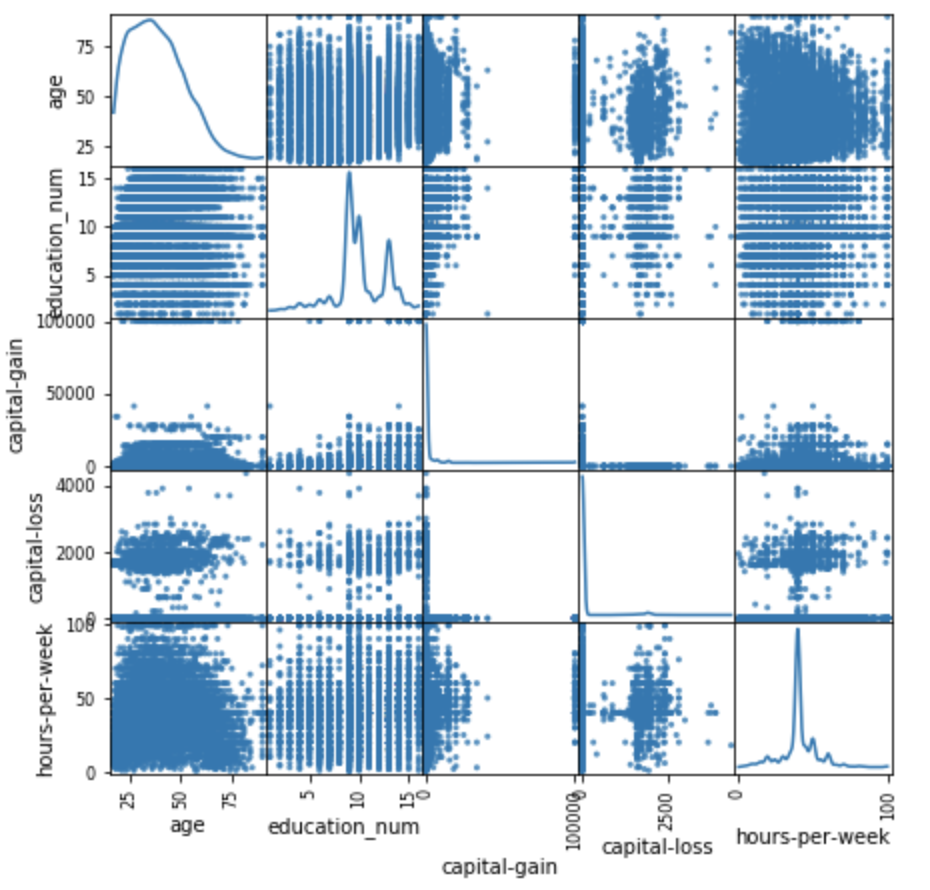
\includegraphics[width=\columnwidth]{images/scatter-matrix.png}
  \caption{Scatter Matrix Plot \cite{Borga2017}.}\label{fig:scatter}
\end{figure}

\par Furthermore, we also explore the capital gains, capital losses, and hours per week variables which we used a histogram to plot the data into distribution form so we can see how all these attributes distributed. The reason we do the histogram is we want to see any skewness in our data. As shown in the histogram graphs in Figure \ref{fig:Hist-capital} and  Figure \ref{fig:loss-capital} in capital gains and capital loss we have highly skewed data which can cause issues later on in our algorithms. We apply a logarithmic function to do highly skewed data to less skewed \cite{www-onlinestat}. Using logarithmic functions adds more value to data from the interpretable standpoint and ``it helps to meet the assumptions of inferential statistics \cite{www-onlinestat}``.

 \begin{figure}[!ht]
  \centering
      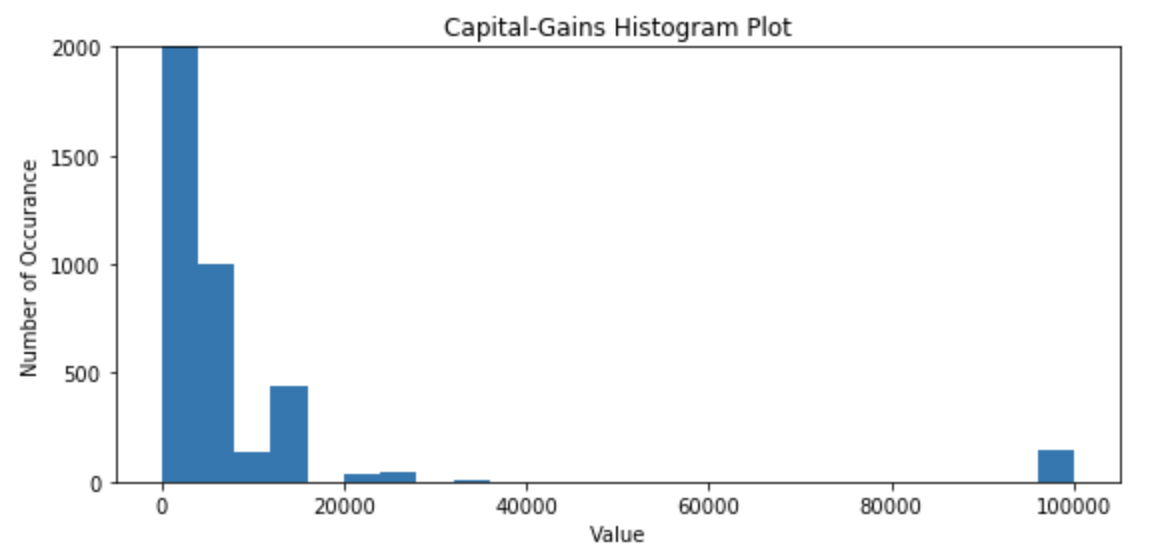
\includegraphics[width=\columnwidth]{images/capital-gain.png}
  \caption{Histogram of Capital Gain \cite{Borga2017}.}\label{fig:Hist-capital}
\end{figure}

 \begin{figure}[!ht]
  \centering
      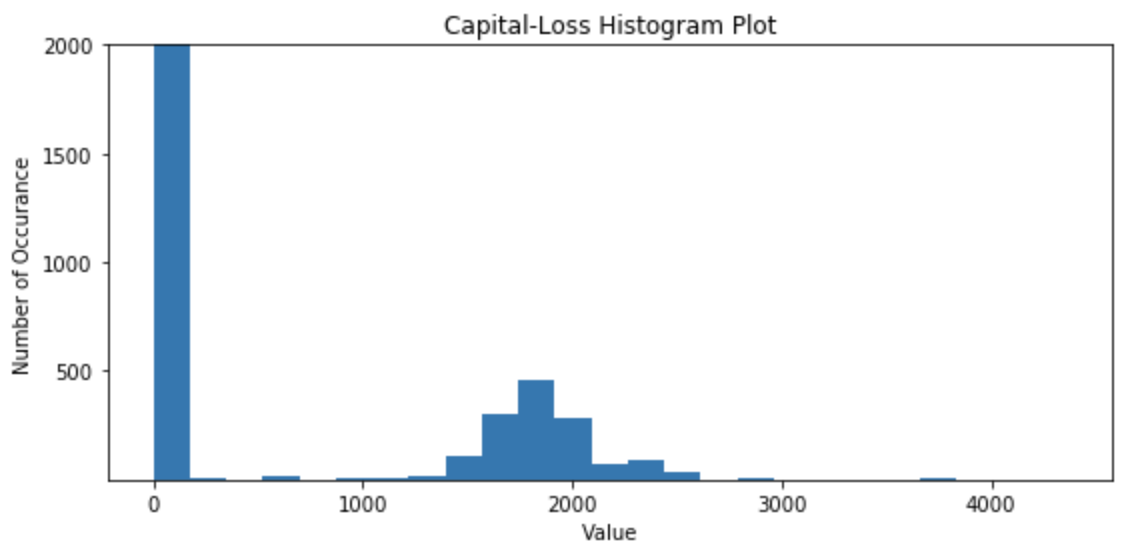
\includegraphics[width=\columnwidth]{images/capital-loss.png}
  \caption{Histogram of Capital Loss \cite{Borga2017}.}\label{fig:loss-capital}
\end{figure}

\par Moreover, applying logarithmic function had an impact on distribution. We can see the changes on skew data in Figure \ref{fig:Hist-capital-log} after applying logarithmic function. 

 \begin{figure}[!ht]
  \centering
      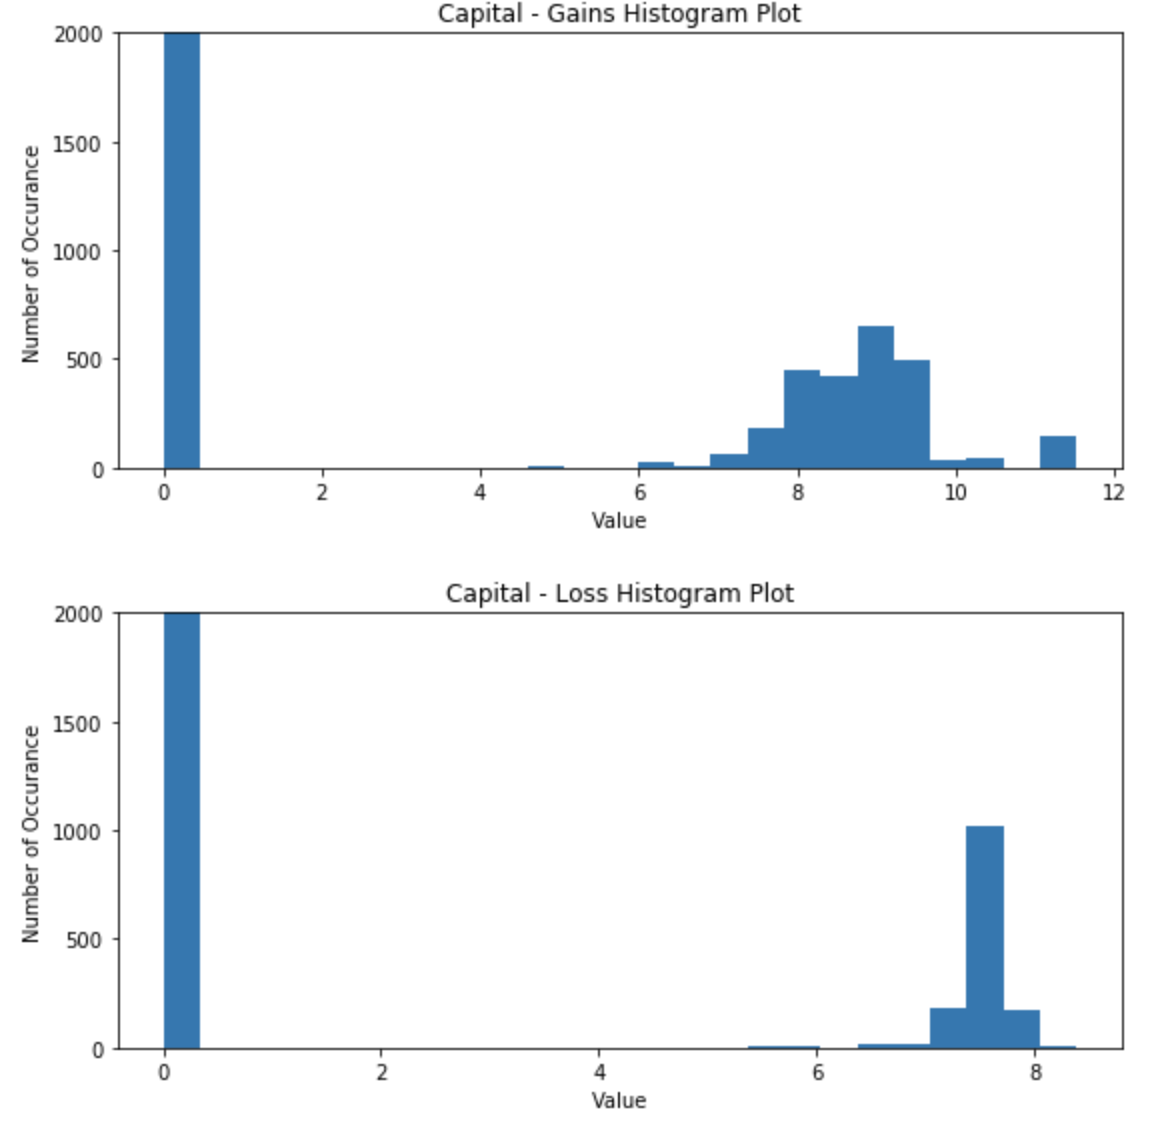
\includegraphics[width=\columnwidth]{images/logarithmic-applied.png}
  \caption{After Logarithmic Function Applied Histogram of Capital Gain \cite{Borga2017}.}\label{fig:Hist-capital-log}
\end{figure}

 

%%%%%%%%%%%%%%%%%%%%%%%%%%%%%%%%%%%%%%%%%%%%%%%%%%%%%%%%%%%%%%%%%%%%%%%%%%%%%%%%%%%%%%%%%%%%%%%%%%%%%%%%%%%%%%%%%%%%%%%%%%%%%%%%%%%%%%%%%%%%%%%%%%%%%%%%%

\section{Machine Learning Algorithms to Consider}
We have multiple algorithms to consider when we are doing the supervised learning. Each algorithm has its benefits and drawbacks. We will consider several supervised machine learning algorithms for our predictions. The application we will use to implement these algorithms will be Python Scikit-Learn library. We will briefly explain each parameter included in these algorithms in Scikit-Learn.

\par First we`ll look at the Scikit-Learn in Python framework we will go through the advantages in Scikit-Learn how we can implement any machine learning in just couple of simple line of codes in Scikit-Learn. 

\subsection{Why Scikit-Learn?}
Scikit-learn developed by David Cournapeau in 2007. The development came from while he was working on summer code project for Google. After recognized and published by INRIA in 2010 project start the get more attention among worldwide. There are more than 30 active contributors and has secured several sponsorships from big technology companies\cite{www-machinelearningmystery}. ``It also has a goal of providing common algorithms to Python users through consistent interface\cite{www-oreily}``. Scikit-Learn consists of several elements to make analytical predictions. These elements are shown below\cite{www-analyticvidhya}:


\par \textbf{Supervised Learning Algorithms:} One of the most fundamental reason that Scikit-Learn's popularity comes from highly available supervised learning algorithms. These algorithms vary from regression models to decision trees and many more\cite{www-analyticvidhya}. 
\par \textbf{Cross Validation:} Scikit-Learn includes various techniqu\-es to check the accuracy or any statistical measure between training and unseen testing set\cite{www-analyticvidhya}. 
\par \textbf{Unsupervised Learning Algorithms:} Scikit-Learn had al\-so various algorithms to support many unsupervised algorithms some of these include clustering, factor analysis, and neural network analysis\cite{www-analyticvidhya}. 
\par \textbf{Various example data-sets:} Scikit-Learn comes with different data sets included in its package so users can start learning Scikit-Learn without the need of any data-sets\cite{www-analyticvidhya}. 
\par \textbf{Feature extraction:} It has rich feature for extracting images or text from data-sets\cite{www-analyticvidhya}.


\par Algorithms that we will investigate shown below; we will go more deep analysis on each of these algorithms. 

\begin{itemize}
    \item Gaussian Naive Bayes
    \item Logistic Regression
    \item K-Nearest Neighbors (KNN)
    \item Stochastic Gradient Descent Classifier
    \item Support Vector Machines
    \item Decision Trees
\end{itemize}

\subsection{Gaussian Naive Bayes}
Naive Bayes bring many beneficial features; it is widely popular among machine learning applications\cite{tapan-kumar}. The popularity of Naive Bayes comes from being able to handle large projects and data-sets faster than most algorithms\cite{tapan-kumar}. It also can handle complex data-sets with categorical and non-categorical inputs \cite{tapan-kumar}. Naive Bayes based on probabilistic classifier of Bayesian theory. It is also a favorite way of doing text categorization \cite{www-wikipedia-naivebayes}. 

\par Term naive comes from it is the method of use probability among categories which assumes of independence among given class of attributes as shown in Figure \ref{fig:Naive Bayes}. In other words, if we try to classify individuals from their email communications it will not take the order of words into account. Whereas in the English language we can tell the difference between sentence makes sense or not if we randomly re-order our words in the sentences. So it does not understand the text, it only looks at word frequencies as a way to do the classification. This is why it is called ``Naive``.  

 \begin{figure}[!ht]
    \centering
    \graphicspath{{images/}}
    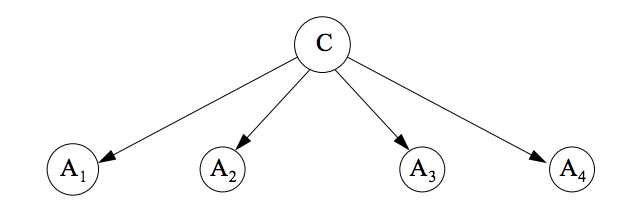
\includegraphics[width=\columnwidth]{Naive-bayes}
    \caption{Example of Naive Bayes \cite{Zhang}.}\label{fig:Naive Bayes}
\end{figure}


\par As we state above Naive Bayes derives from Bayesian Theory where the dimensionality of inputs is relatively high. Bayesian Theorem is stated below \cite{Sayali}.

\begin{equation}
P(C \mid X) = \frac{P(X \mid C) \times P(C)} {P(X)}
\end{equation}

Naive Bayes Classifier works as follows \cite{Sayali}:

\textbf{Advantages of Naive Bayes \cite{Sayali}:}
\begin{itemize}
\item Faster classification time for training data-set.
\item Because of independent classification it improves classification performance.
\item Performance is relatively good. 
\end{itemize}

\textbf{Disadvantages of Naive Bayes\cite{Sayali}:}

\begin{itemize}
\item Often it requires a large number of data-sets to give adequate results.
\item On some occasions which are relative to data-sets, it can give less accuracy.
\end{itemize}

\subsection{Logistic Regression}

Logistic Regression widely used for predicting ``probability of failure in a given system, product, and process \cite{adarsh}``. Logistic Regression also used in natural language analysis, it is an extension of conditional random fields \cite{adarsh}. It works as a classifier which learns the features from the input given and classifies them by multiplying the input value with the weight value \cite{tweet-logistic}.

\begin{equation}
P(C \mid X) = \sum_{i=1}^{N} W_i \times f_i 
\end{equation}

\par Main reason that Logistic Regression differs from Linear Regression is output variable for Logistic Regression is binary whereas output variable in Linear Regression is discrete(continuous) \cite{fang-logistic}. 

\textbf{Advantages of Logistic Regression:}
\begin{itemize}
\item It does not have any assumptions over distribution of classes \cite{www-washington}.
\item It is fast to train \cite{www-washington}.
\item Logistic Regression has fast classifying method of unknown data \cite{www-washington}.
\item We can easily extend to other regression for multiple classes like multinomial regression \cite{www-washington}. 
\end{itemize}

\textbf{Disadvantages of Logistic Regression:}

\begin{itemize}
\item One of the disadvantages of linear regression is it is not providing flexibility in some instances. What we mean by the `` lack of flexibility is the linear dependency, and linear decision boundary in the instance space is not valid \cite{www-old.cs}``. This disadvantage can be improved changing from Logistic Regression to Choquistic Regression\cite{www-old.cs}.
\item Logistic regression can provide poor results when there are more complex relationships in data \cite{www-elitedatascience}.
\item Logistic models also have over-fitting problems which come from a result of sampling bias \cite{www-classroom}.
\item Because of Logistic Regression's predictions comes from the independent variable if the researcher includes wrong independent variables then model's prediction will have no value \cite{www-classroom}.
\item Because it is predictions based on 1 and 0 model will have poor performance when predicting continuous variables \cite{www-classroom}. 
\end{itemize}


\subsection{K-Nearest Neighbors (KNN)}
K Nearest neighbor has been primarily studied, and this popularity comes from it has been applied to many applications some of these applications are ``spatial databases, pattern recognition, geographic information, image retrieval, computer game, and many other applications \cite{Lee2017-knn}``. Due to an increase of mobile devices and people tends to use of applications like navigation K-nearest neighbor found itself another widely used area of location-based services due to an ability to found a target location \cite{Lee2017-knn}. 

\par Intuition behind the K Nearest Neighbor can be described as follows: `` for a set P of n objects and a querying point q, return the k objects in P that are closest to q \cite{Lee2017-knn}.``


\textbf{Advantages of K Nearest Neighbors:}
\begin{itemize}
\item K Nearest Neighbor is a basic and simple approach to implement \cite{www-cs.man}.
\item K Nearest Neighbor can perform well and efficiently with the large amount of data \cite{www-revoledu}.
\item K nearest Neighbor also does effectively well with noisy data sets (``if the inverse square of weighted distance used as the distance \cite{www-revoledu}``). In other words, it is flexible to feature and distance choices \cite{www-cs.man}.
\end{itemize}

\textbf{Disadvantages of K Nearest Neighbors:}

\begin{itemize}
\item K Nearest Neighbor typically require large dataset to perform well \cite{www-cs.man}. 
\item Time complexity could be high due to computing distance of each query to all training data points \cite{www-revoledu}. This time might be improved with some indexing (K-D Tree) \cite{www-revoledu}.
\item Determining the value of K can be time-consuming \cite{www-revoledu}. 
\item It can be unclear to know which type of distance to use, as well as which variability to use to get the optimal results \cite{www-revoledu}. 
\item Switching the different K values can result in the predicted class labels \cite{www-nickgillian}. 
\end{itemize}

Many of these disadvantages are improving with the help of parallel distributed computing. Recent improvements in MapReduce framework allows users to run KNN algorithms in the cluster which had a significant effect on reducing the computation time \cite{knn-chung}.

\par Another area of improvements on KNN, is to implement different mapping functions such as kernel KNN, kernel difference weighted KNN, adaptive quasi-conformal kernel nearest neighbor, angular similarity, local linear discriminant analysis, and Dempster-Shafer \cite{ERTUGRUL2017480}. 

\subsection{Decision Trees}
 
Decision Tree is another widely used algorithm model for classification and regression. Decision Trees uses a recursive split model where each recursive split is identified by each data point; this is an example of non-parametric hierarchical model \cite{HASSAN201752}. 
\par Representation of decision trees is as follows; we sort the instances from root to leaf nodes, this sorting gives insights about the classification of the instance, every outcome descending from the root node corresponds to possible values for that variable \cite{www-cs.princeton}. We can classify an instance by starting from the root node and checking the attributes labeled on that node and moving down from that node based on attribute given attribute values \cite{www-cs.princeton} as shown in Figure \ref{fig:Decision Tree}. 

 \begin{figure}[!ht]
  \centering
      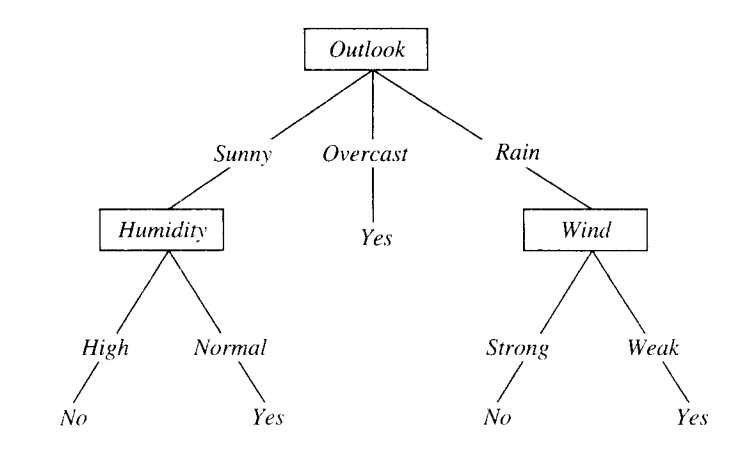
\includegraphics[width=\columnwidth]{images/decison_tree.png}
  \caption{Example of Decision Tree Construction\cite{www-cs.princeton}.}\label{fig:Decision Tree}
\end{figure}

\textbf{Advantages of Decision Trees:}

\begin{itemize}
\item Decision Tree applications are easy to interpret and understand \cite{www-cs.ubb}. This ease comes from their schematic representation \cite{www-cs.ubb}. Interpretation between alternatives can be expressed with single numerical number which is the expected value (EV) \cite{www-cs.ubb}.  
\item Decision Trees can handle noisy or incomplete data-sets \cite{www-cs.ubb}. In other words it requires little effort of data preparation because of it is flexibility \cite{www-simafore}.  
\item It can handle both nominal and numerical variables \cite{www-cs.ubb}.
\item It can be modified easily whenever the new information is available \cite{www-cs.ubb}.
\item 
\end{itemize}


\textbf{Disadvantages of Decision Trees:}

\begin{itemize}
\item Because of it is a use of divide and conquer method they can demonstrate good performance if there are few attributes exists when the attributes level goes into large number decision tree become more complex which will result in poor performance \cite{www-cs.ubb}.
\item Decision Trees are also susceptible to training set which can give a result of over-fitting \cite{www-cs.ubb}. In other words, it can believe the training set completely which will give an abysmal performance on testing set.
\item ID3 and C4.5 decision tree algorithms require discrete values as input data. 
\end{itemize}

\subsection{Stochastic Gradient Descent Classifier (SGD)}

Stochastic Gradient Descent recently got became more popular because of it is large-scale learning ability in machine learning problems \cite{fan-stochastic}. It is a useful and straightforward way approach of linear classifiers under convex problems which is Support Vector Machines or Conditional Random Fields \cite{www-bottou}. The originality of SGD derives from ``Stochastic Approximation`` which is a work from Robinson and Manroe \cite{Needell2016}. 

\textbf{Advantages of Stochastic Gradient Descent:}

\begin{itemize}
\item One of the advantage of stochastic gradient descent is, it is easy to implement \cite{www-scikit-stochastic-gradient}.
\item Stochastic Gradient Descent is also efficient because of each step only relies on a single derivative which makes the computational cost  {1} / {n} than normal gradient descent \cite{NIPS2013_4937}.
\end{itemize}

\textbf{Disadvantages of Stochastic Gradient Descent:}

\begin{itemize}
\item Stochastic Gradient Descent can be required to have many iterations, and it also requires some hyper-parameters \cite{www-scikit-stochastic-gradient}. 
\item Feature scaling is a practice which used in the standardization of range of independent variables \cite{www-wikipedia-futurescaling}. SGD also used this feature scaling technique and it can be sensitive to feature scaling \cite{www-scikit-stochastic-gradient}. 
\item Another drawback of Stochastic Gradient Descent is while using GPU they are hard to parallelize or distributing them using computer clusters \cite{andrewng-deeplearning}. 
\end{itemize}




\subsection{Support Vector Machines}
Support Vector Machines is fallen under the classification methods in machine learning \cite{www-simafore-svm}. It is also a robust classification method that has been widely found itself an area ranging from pattern recognition to text analysis \cite{www-simafore-svm}. 
\par Fitting a boundary between data points is the principle of the support vector machines. This boundary divides the data points between classes, and each similar data point puts under the same class classification \cite{www-simafore-svm}. After training the support vector machines with training data-set, we only need to check whether the test data lies under the boundaries for testing set. Another thing to consider is after it creates the boundaries of the data remaining training data becomes obsolete because we only need the core set of points which supports the boundaries to classify the new data set. This core data points called ``support vectors``. It is called vector because of each data point contains a row of observed data values for attributes \cite{www-simafore-svm}. 

 \begin{figure}[!ht]
  \centering
      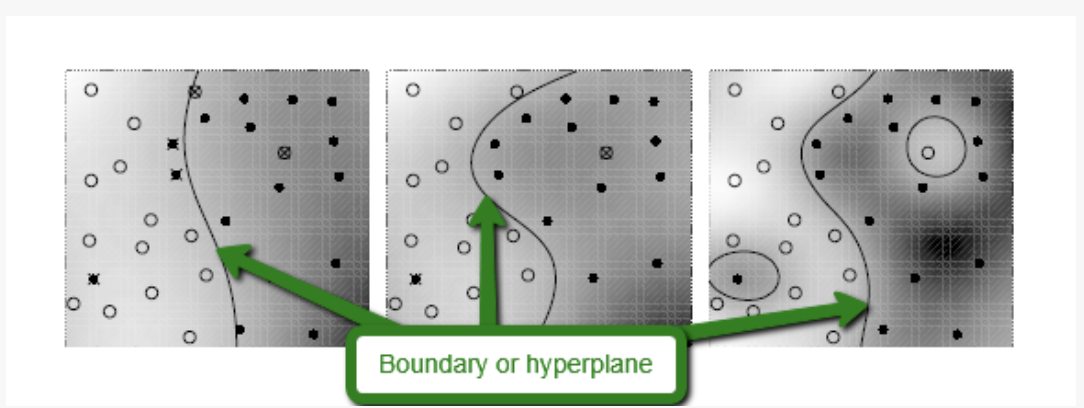
\includegraphics[width=\columnwidth]{images/hyperplane-boundary.png}
  \caption{Example of Shows the Hyperplanes \cite{www-simafore-svm}.}\label{fig:Hyperplane}
\end{figure}

\par Traditionally boundaries are called ``hyperplanes`` and it is used to describe boundaries in more than three dimensions because they are hard or sometimes impossible to visualize.\cite{www-simafore}. Figure \ref{fig:Hyperplane}. Optimality of hyperplane expressed as a linear function which requires maximum distance between the identified classes. It only considers a small number of training example to build this hyperplane. SVM hyperplanes based on `` separation of positive (+1) and negative (-1) with the largest margin \cite{verma-ssv}``.

\par One of the main characteristic of the machine learning is to generalization. In other words, we want to give a general idea that tends to fit any of our testing datasets optimally. Support vector machines are a perfect regarding generalizations because once the training data fitted by the support vector machines other than support vector data inside the training data becomes redundant which means that even with the small changes inside the data will not have a significant effect on general boundaries \cite{www-simafore-svm}. 

\textbf{Advantages of Support Vector Machines:}
\begin{itemize}
\item Generalizes the data well with the help of boundaries. Which reduces the overfitting \cite{www-simafore-svm}.
\item Classification accuracy in basic support vector machine will yield a 95 percent accuracy with a default settings \cite{www-simafore-svm}. 
\item SVM can deliver a unique solution, because of optimality solution is convex. This will give an advantage over Neural Networks which has multiple solutions in local minima \cite{berlin-svm}.
\end{itemize}

\textbf{Disadvantages of Support Vector Machines:}

\begin{itemize}
\item One common disadvantage of SVM, is the lack of transparency because of its non-parametric techniques \cite{berlin-svm}.
\item Another biggest disadvantage of SVM is it requires high algorithmic complexity and high level of memory for the large-scale implementations \cite{verma-ssv}. 
\item According to Burgees, biggest limitation of the SVM is in the choice of kernel \cite{Burges1998}.
\end{itemize}

\subsection{Ensemble Methods}
Ensemble methods goes into classification algorithm category, they are learning algorithms which uses weighted vote for it is prediction methods, in other words, it is learning rules over a small subset of data then we combine these rules which we learn from the small subset of data to make predictions and/or classification on the testing data \cite{dietterich-ensemble}. The originality of the Ensemble method comes from Bayesian averaging, but with the recent algorithms include ``Bagging, error-correcting, and boosting \cite{dietterich-ensemble}``. 

\par Bagging refers to simply the looking at data-sets and dividing the data-set to it is small subsets then learning the rules of that particular small subset. Next step is combining each learned rule from subsets to apply to more significant data set. Combining method mostly done with averaging the learned rules. Bagging also does better on testing set than standard Linear Regression analysis and linear regression does better on training set especially in third order polynomial \cite{dietterich-ensemble}.  

\par Stacking 

\par Boosting is another method used in Ensemble Methods. The difference from bagging is in boosting we need to pick subsets or examples that we are not good at in other words hardest examples. Then we combine these learned rules with the weighted mean instead mean used in bagging method. 

\par Boosting is little different then bagging. 

\textbf{Advantages of Ensemble Methods:} 
\begin{itemize}
\item Prediction of the ensemble methods is better than most of the algorithms because of the combining methods intuition makes the model less noisy \cite{www-ensembleanalyticvidhya}. 
\item They are more stable than other algorithms. \cite{www-ensembleanalyticvidhya}
\end{itemize}

\textbf{Disadvantages of Ensemble Methods:}
\begin{itemize}
\item Over-fitting may cause some disadvantages for ensemble learning but bagging operation will reduce this overfitting \cite{www-ensembleanalyticvidhya}. 
\end{itemize}


\section{Fitting Data Into Machine Learning Algorithms}

In this section, we will show the techniques we used on the execution of the prepared data into machine learning algorithms. Before fitting the data into the machine learning algorithms, we split the data into two sets. These sets are the training set and the testing set. We do splitting because of gaining an access of the future data will most likely be hard before future occurs, and because of this fact, it is a good idea to test our model with a dataset which our model has not seen it \cite{www-salford}. 
\par We used scikit-learn for splitting data into train and test we saved 20\% of data for testing purposes as shown in Table \ref{split} . 

\begin{table}[!ht]
\centering
\begin{tabular}{|l|l|}
\hline
\textbf{Splitting the Data} & \textbf{Sample Size} \\ \hline
Training                    & 24129                \\ \hline
Testing                     & 6033                 \\ \hline
\end{tabular}
\caption{Train-Test-Split \cite{Borga2017}.}
\label{split}
\end{table}

\par Furthermore, after splitting the data we put all of our training data into to each of the machine learning algorithm to get their prediction results. We also provided code at the beginning and the end of each algorithm to calculate their running time.

\par Before we move further we need to discuss critical characteristics of a machine learning algorithm. These are;

\begin{itemize}
    \item Confusion Matrix
    \item Accuracy
    \item Recall
    \item F-1 Score
    \item Precision 
\end{itemize}

\subsubsection{\textbf{Confusion Matrix:}}
Confusion matrix develops from 4 key elements. These elements are true positive, true negative, false negative, and false positive. As shown in Figure \ref{fig:confusion-matrix} about the constructing a confusion matrix. If we want to build a confusion matrix by targeting individuals who are making more than \$50K our true positive, true negative, false positive, and false negative explained below. 

\begin{figure}[!ht]
  \centering
      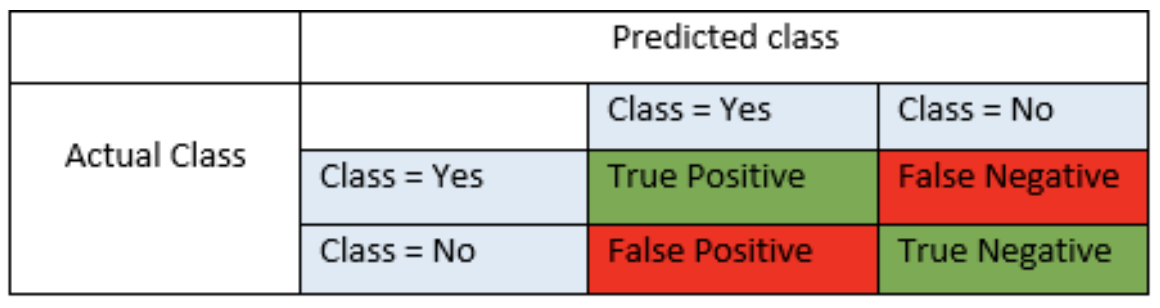
\includegraphics[width=\columnwidth]{images/confusion-matrix.png}
  \caption{Example of Confusion Matrix Construction \cite{www-exsilio}.}\label{fig:confusion-matrix}
\end{figure}

\par \textbf{True Positive (TP):} We can explain true positive as if the individuals make more than \$50K and our model correctly classifies them as individuals who makes more than \$50K, then this individual is in higher income range, in this case, we call it a true positive \cite{www-exsilio}. 

\par \textbf{True Negative (TN):} Intuition of true negative is if an individual makes less than \$50K and our model correctly classifies them as individuals who makes less then \$50K, then this individual is in lower income range. We call this true negative \cite{www-exsilio}. 

\par \textbf{False Negative (FN):} When an individual makes less than \$50K and our model incorrectly classifies them in higher income range by making a mistake causes a false negative to happen \cite{www-exsilio}.

\par \textbf{False Positive (FP):} When an individual is making more than \$50K and our model classifies them in lower income range by mistake. This is called false positive \cite{www-exsilio}. 

\subsubsection{\textbf{Accuracy:}}
Accuracy answers the question of how good is the model is. In our case this question will be out of all the individuals, how many did the models classify the individuals correctly. The mathematical expression of the accuracy is the ratio between the number of correctly classified points and the number of total points. We can think that if we have high accuracy, our model is excellent, but this is only where we have identical false positive and false negative values in our dataset \cite{www-exsilio}.

\begin{equation}
Accuracy = \frac{TP + TN} {TP + FP + FN + TN}
\end{equation}

\subsubsection{\textbf{Precision}}
Precision answers the questions of out of all the points predicted to be positive how many of them were actually positive? If we translate this question into our case, we will have out of all the individuals that we are classified as lower income how many were actually have lower income. Higher precision indicates that we have low false positive rate \cite{www-exsilio}. Mathematical expression of precision is; 

\begin{equation}
Precision = \frac{TP} {TP + FP}
\end{equation}

\subsubsection{\textbf{Recall (Sensitivity)}}

Recall answers the question of ``out of the points that are labeled positive how many of them were correctly predicted is positive ? ``. If we translate this to our case, we will have ``out of the points that are labeled higher income how many of them correctly predicted is in higher income range ? ``. Mathematical expression of the recall is; 

\begin{equation}
Precision = \frac{TP} {TP + FN}
\end{equation}

\subsubsection{\textbf{F-1 Score}}

The F-1 score is the idea of giving a decision by looking at only one score which will include precision, and recall scores. We cannot just take the average of precision and recall because if either of them is very low. We need a number to be low, even id the other one is not. This will leads us to look at the harmonic mean, and it works as follow. Let's say we have two numbers X and Y. X is smaller than Y, and we have the arithmetic mean, and it always lies between X and Y. It is a mathematical fact that the harmonic mean is always less than the arithmetic mean which is closer to the smaller number than to the higher number. Mathematical expression of F-1 score is; 

\begin{equation}
F1 Score = 2 \times {\frac{Precision \times Recall} {Precision + Recall}}
\end{equation}

\subsection{Results}
Now we can look at the results from each of the machine learning algorithm. Results also showed in Table \ref{result-table} with the visualization of Figure \ref{fig:result-algo}. We can also see the running time of the each of the algorithm in Figure \ref{fig:result-time}. Support Vector Machines is the winner for the highest running time for training the algorithm. 

\begin{figure}[!ht]
  \centering
      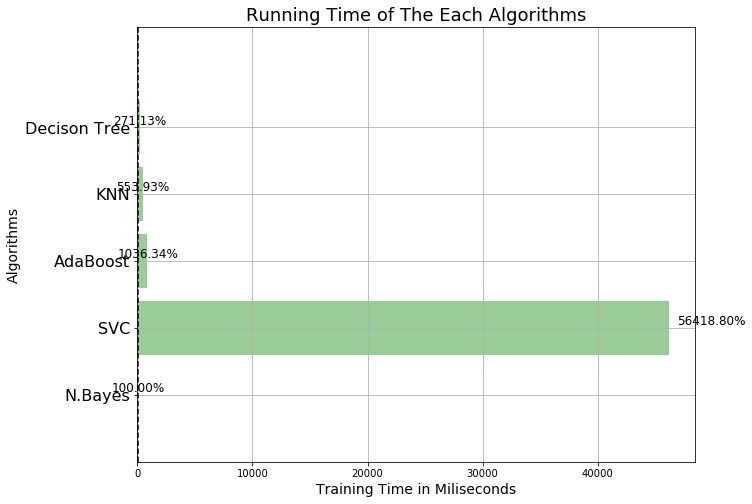
\includegraphics[width=\columnwidth]{images/running-time.png}
  \caption{Supervised Learning Algorithm Running Time Results \cite{Borga2017}.}\label{fig:result-time}
\end{figure}

\begin{table}[!ht]
\centering
\begin{tabular}{lllll}
\hline
Name                                & Accuracy                    & Recall                      & Precision                   & F1 Score                    \\ \hline
\multicolumn{1}{|l|}{Naive Bayes}   & \multicolumn{1}{l|}{0.4442} & \multicolumn{1}{l|}{0.4642} & \multicolumn{1}{l|}{0.9680} & \multicolumn{1}{l|}{0.3053} \\ \hline
\multicolumn{1}{|l|}{SVC}           & \multicolumn{1}{l|}{0.8301} & \multicolumn{1}{l|}{0.5969} & \multicolumn{1}{l|}{0.5056} & \multicolumn{1}{l|}{0.7284} \\ \hline
\multicolumn{1}{|l|}{AdaBoost}      & \multicolumn{1}{l|}{0.8499} & \multicolumn{1}{l|}{0.6724} & \multicolumn{1}{l|}{0.6189} & \multicolumn{1}{l|}{0.7361} \\ \hline
\multicolumn{1}{|l|}{KNN}           & \multicolumn{1}{l|}{0.8184} & \multicolumn{1}{l|}{0.6090} & \multicolumn{1}{l|}{0.5682} & \multicolumn{1}{l|}{0.6561} \\ \hline
\multicolumn{1}{|l|}{Decision Tree} & \multicolumn{1}{l|}{0.8161} & \multicolumn{1}{l|}{0.6231} & \multicolumn{1}{l|}{0.6109} & \multicolumn{1}{l|}{0.6459} \\ \hline
\end{tabular}
\caption{Results of the Algorithms \cite{Borga2017}.}
\label{result-table}
\end{table}

\subsubsection{\textbf{Naive Bayes}} 
As shown in the Figure \ref{fig:result-algo} we have a comparison of several supervised machine learning algorithms on our dataset. We can see that from the accuracy standpoint Naive Bayes algorithms have the lowest score which means that it did not do a good job for labeling true positives regards to all data but it did a good job in precision standpoint while doing a bad classification from recall standpoint. Two key element for us in this situation is accuracy and f1 score(which consist of precision and recall). 
\subsubsection{\textbf{Support Vector Machine}}
Support Vector Machine is the second best algorithm in our case. This algorithm did very well job on classification it has the second highest accuracy and f1 score. 
\subsubsection{\textbf{AdaBoost}}
As we stated before ensemble algorithms learn from the small portion of the data and combine these learning to do the predictive task. As shown in Figure \ref{fig:result-algo} adaboosting has the highest accuracy score among all the other algorithms. This algorithm should be our first choice to do predictive modeling. We believe that there is still an improvements on accuracy 
\subsubsection{\textbf{K-Nearest Neighboors}}
K-Nearest Neighbor algorithm in our project we set the k value to 5. K Nearest Neighbor algorithm also did a good job by placing itself third in accuracy score. 

\subsubsection{\textbf{Decision Tree}} 
Decision Tree is gave a good accuracy but fall behind on f1 score as shown in Figure \ref{fig:result-algo}.






\begin{figure}[!ht]
  \centering
      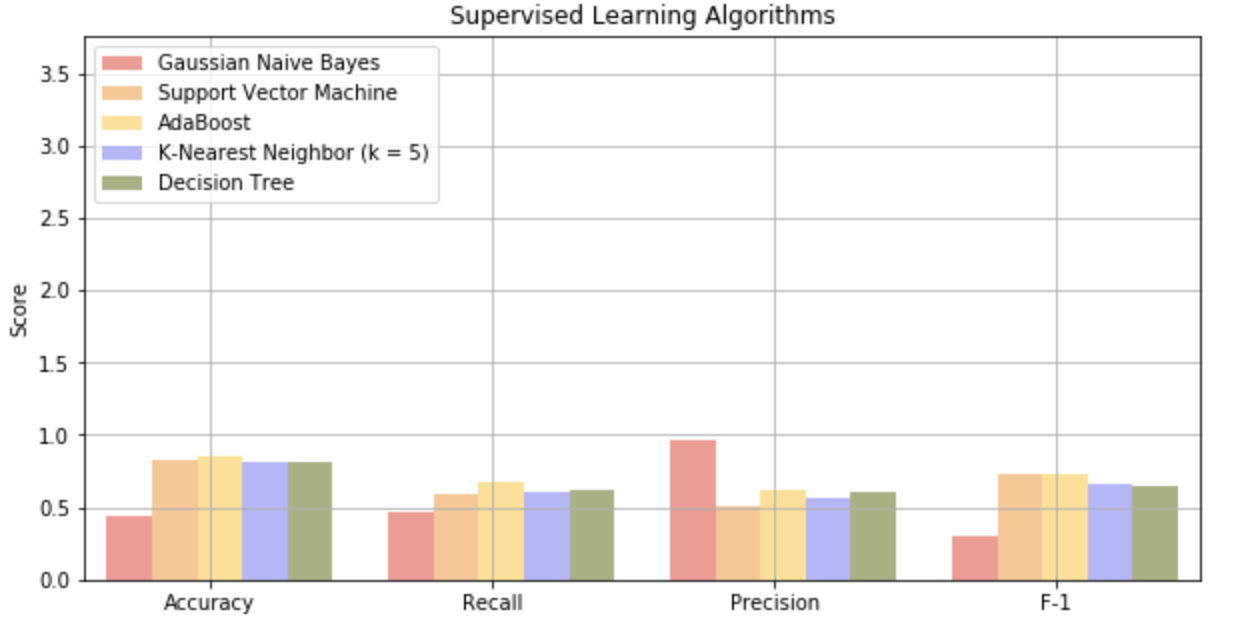
\includegraphics[width=\columnwidth]{images/result-score.png}
  \caption{Supervised Learning Algorithm Results \cite{Borga2017}.}\label{fig:result-algo}
\end{figure}

%%%%%%%%%%%%%%%%%%%%%%%%%%%%%%%%%%%%%%%%%%%%%%%%%%%%%%%%%%%%%%%%%%%%%%%%%%%%%%%%%%%%%%%%%%%%%%%%%%%%%%%%%%%%%%%%%%%%%%%%%%%%%%%%%%%%%%%%%%%%%%%%%%%%%%%%%

\section{Conclusion}

We presented the importance of analytical approach with machine learning algorithms and how they can be used to predict or classify the individuals with many different attributes like age, education, income, etc. We also presented weaknesses and strengths of these algorithms along with their precision, accuracy, recall, and F-1 scores by presenting with the visualizations. We also demonstrated the running time for each algorithm while using big data sets. The source code of this project can found Github website which presented in reference section \cite{Borga2017}.





\begin{acks}

The author would like to thank Dr. Gregor von Laszewski for his support and suggestions to write this paper.

\end{acks}

\bibliographystyle{ACM-Reference-Format}
\bibliography{report} 



\end{document}
